\documentclass[a4paper]{book}
\usepackage{makeidx}
\usepackage{natbib}
\usepackage{graphicx}
\usepackage{multicol}
\usepackage{float}
\usepackage{listings}
\usepackage{color}
\usepackage{ifthen}
\usepackage[table]{xcolor}
\usepackage{textcomp}
\usepackage{alltt}
\usepackage{ifpdf}
\ifpdf
\usepackage[pdftex,
            pagebackref=true,
            colorlinks=true,
            linkcolor=blue,
            unicode
           ]{hyperref}
\else
\usepackage[ps2pdf,
            pagebackref=true,
            colorlinks=true,
            linkcolor=blue,
            unicode
           ]{hyperref}
\usepackage{pspicture}
\fi
\usepackage[utf8]{inputenc}
\usepackage{mathptmx}
\usepackage[scaled=.90]{helvet}
\usepackage{courier}
\usepackage{sectsty}
\usepackage[titles]{tocloft}
\usepackage{doxygen}
\lstset{language=C++,inputencoding=utf8,basicstyle=\footnotesize,breaklines=true,breakatwhitespace=true,tabsize=8,numbers=left }
\makeindex
\setcounter{tocdepth}{3}
\renewcommand{\footrulewidth}{0.4pt}
\renewcommand{\familydefault}{\sfdefault}
\hfuzz=15pt
\setlength{\emergencystretch}{15pt}
\hbadness=750
\tolerance=750
\begin{document}
\hypersetup{pageanchor=false,citecolor=blue}
\begin{titlepage}
\vspace*{7cm}
\begin{center}
{\Large \-My \-Project }\\
\vspace*{1cm}
{\large \-Generated by Doxygen 1.7.6.1}\\
\vspace*{0.5cm}
{\small Sat Aug 16 2014 13:12:32}\\
\end{center}
\end{titlepage}
\clearemptydoublepage
\pagenumbering{roman}
\tableofcontents
\clearemptydoublepage
\pagenumbering{arabic}
\hypersetup{pageanchor=true,citecolor=blue}
\chapter{\-Class \-Index}
\section{\-Class \-Hierarchy}
\-This inheritance list is sorted roughly, but not completely, alphabetically\-:\begin{DoxyCompactList}
\item \contentsline{section}{\-Animation}{\pageref{structAnimation}}{}
\item \contentsline{section}{\-Board\-Column}{\pageref{classBoardColumn}}{}
\item \contentsline{section}{\-Connect\-Four\-Object}{\pageref{classConnectFourObject}}{}
\begin{DoxyCompactList}
\item \contentsline{section}{\-Connect\-Four\-Render\-Object}{\pageref{classConnectFourRenderObject}}{}
\begin{DoxyCompactList}
\item \contentsline{section}{\-Game\-Board\-Renderer}{\pageref{classGameBoardRenderer}}{}
\item \contentsline{section}{\-Game\-Coin\-Renderer}{\pageref{classGameCoinRenderer}}{}
\end{DoxyCompactList}
\item \contentsline{section}{\-Game\-Board}{\pageref{classGameBoard}}{}
\end{DoxyCompactList}
\item \contentsline{section}{\-Game}{\pageref{structGame}}{}
\item \contentsline{section}{\-Game\-Database}{\pageref{classGameDatabase}}{}
\item \contentsline{section}{\-Game\-Manager}{\pageref{classGameManager}}{}
\begin{DoxyCompactList}
\item \contentsline{section}{\-A\-I\-Game\-Manager}{\pageref{classAIGameManager}}{}
\item \contentsline{section}{\-T\-C\-P\-Game\-Manager}{\pageref{classTCPGameManager}}{}
\end{DoxyCompactList}
\item \contentsline{section}{\-Game\-Over\-Screen}{\pageref{classGameOverScreen}}{}
\item \contentsline{section}{\-Game\-Renderer}{\pageref{classGameRenderer}}{}
\item \contentsline{section}{\-Game\-Results}{\pageref{classGameResults}}{}
\item \contentsline{section}{\-Helper}{\pageref{classHelper}}{}
\item \contentsline{section}{\-Main\-Window}{\pageref{classMainWindow}}{}
\item \contentsline{section}{\-Min\-Max}{\pageref{classMinMax}}{}
\item \contentsline{section}{\-Network\-Adapter}{\pageref{classNetworkAdapter}}{}
\begin{DoxyCompactList}
\item \contentsline{section}{\-Game\-Client}{\pageref{classGameClient}}{}
\item \contentsline{section}{\-Game\-Server}{\pageref{classGameServer}}{}
\end{DoxyCompactList}
\item \contentsline{section}{\-Player}{\pageref{classPlayer}}{}
\item \contentsline{section}{\-Render\-Object}{\pageref{classRenderObject}}{}
\begin{DoxyCompactList}
\item \contentsline{section}{\-Connect\-Four\-Render\-Object}{\pageref{classConnectFourRenderObject}}{}
\end{DoxyCompactList}
\item \contentsline{section}{\-Settings}{\pageref{structSettings}}{}
\item \contentsline{section}{\-Settings\-Widget}{\pageref{classSettingsWidget}}{}
\end{DoxyCompactList}

\chapter{\-Class \-Index}
\section{\-Class \-List}
\-Here are the classes, structs, unions and interfaces with brief descriptions\-:\begin{DoxyCompactList}
\item\contentsline{section}{\hyperlink{classAIGameManager}{\-A\-I\-Game\-Manager} \\*\-Ai specific gamemanager }{\pageref{classAIGameManager}}{}
\item\contentsline{section}{\hyperlink{structAnimation}{\-Animation} \\*\-Handles animation state }{\pageref{structAnimation}}{}
\item\contentsline{section}{\hyperlink{classBoardColumn}{\-Board\-Column} \\*\-Column for the game board }{\pageref{classBoardColumn}}{}
\item\contentsline{section}{\hyperlink{classConnectFourObject}{\-Connect\-Four\-Object} \\*\-Base class for every connect four related class }{\pageref{classConnectFourObject}}{}
\item\contentsline{section}{\hyperlink{classConnectFourRenderObject}{\-Connect\-Four\-Render\-Object} \\*\-Base class for each renderable connect four object }{\pageref{classConnectFourRenderObject}}{}
\item\contentsline{section}{\hyperlink{structGame}{\-Game} \\*\-Data holder for game results }{\pageref{structGame}}{}
\item\contentsline{section}{\hyperlink{classGameBoard}{\-Game\-Board} \\*\hyperlink{structGame}{\-Game} board class representing game board }{\pageref{classGameBoard}}{}
\item\contentsline{section}{\hyperlink{classGameBoardRenderer}{\-Game\-Board\-Renderer} \\*\-Class that is responsible for rendering the gameboard }{\pageref{classGameBoardRenderer}}{}
\item\contentsline{section}{\hyperlink{classGameClient}{\-Game\-Client} \\*\-Class that is responsible for opening a tcp socket connection to the host }{\pageref{classGameClient}}{}
\item\contentsline{section}{\hyperlink{classGameCoinRenderer}{\-Game\-Coin\-Renderer} \\*\-Class that is responsible for rendering the coins added to the board }{\pageref{classGameCoinRenderer}}{}
\item\contentsline{section}{\hyperlink{classGameDatabase}{\-Game\-Database} \\*\-Singleton class that manages the game result database }{\pageref{classGameDatabase}}{}
\item\contentsline{section}{\hyperlink{classGameManager}{\-Game\-Manager} \\*\-Class that handles game states and instanciates renderer and board }{\pageref{classGameManager}}{}
\item\contentsline{section}{\hyperlink{classGameOverScreen}{\-Game\-Over\-Screen} \\*\-Class that handles game over screen }{\pageref{classGameOverScreen}}{}
\item\contentsline{section}{\hyperlink{classGameRenderer}{\-Game\-Renderer} \\*\-Handles \-Open\-G\-L window inside main window; }{\pageref{classGameRenderer}}{}
\item\contentsline{section}{\hyperlink{classGameResults}{\-Game\-Results} \\*\-Show previous games }{\pageref{classGameResults}}{}
\item\contentsline{section}{\hyperlink{classGameServer}{\-Game\-Server} \\*\-Class that handles server client connection }{\pageref{classGameServer}}{}
\item\contentsline{section}{\hyperlink{classHelper}{\-Helper} \\*\hyperlink{classHelper}{\-Helper} class for \-Connect \-Four }{\pageref{classHelper}}{}
\item\contentsline{section}{\hyperlink{classMainWindow}{\-Main\-Window} \\*\-Main window class }{\pageref{classMainWindow}}{}
\item\contentsline{section}{\hyperlink{classMinMax}{\-Min\-Max} \\*\-Negamax algorithm }{\pageref{classMinMax}}{}
\item\contentsline{section}{\hyperlink{classNetworkAdapter}{\-Network\-Adapter} \\*\-Base class for a network connection (server and client) }{\pageref{classNetworkAdapter}}{}
\item\contentsline{section}{\hyperlink{classPlayer}{\-Player} \\*\hyperlink{classPlayer}{\-Player} data holder }{\pageref{classPlayer}}{}
\item\contentsline{section}{\hyperlink{classRenderObject}{\-Render\-Object} \\*\-Abstract class for each renderable object }{\pageref{classRenderObject}}{}
\item\contentsline{section}{\hyperlink{structSettings}{\-Settings} \\*\-Data holder between ui and game }{\pageref{structSettings}}{}
\item\contentsline{section}{\hyperlink{classSettingsWidget}{\-Settings\-Widget} \\*\-Widget for settings }{\pageref{classSettingsWidget}}{}
\item\contentsline{section}{\hyperlink{classTCPGameManager}{\-T\-C\-P\-Game\-Manager} \\*\-Gamemanager that handles \-Network game related tasks }{\pageref{classTCPGameManager}}{}
\end{DoxyCompactList}

\chapter{\-Class \-Documentation}
\hypertarget{classAIGameManager}{\section{\-A\-I\-Game\-Manager \-Class \-Reference}
\label{classAIGameManager}\index{\-A\-I\-Game\-Manager@{\-A\-I\-Game\-Manager}}
}


ai specific gamemanager  




{\ttfamily \#include $<$aigamemanager.\-h$>$}

\-Inheritance diagram for \-A\-I\-Game\-Manager\-:\begin{figure}[H]
\begin{center}
\leavevmode
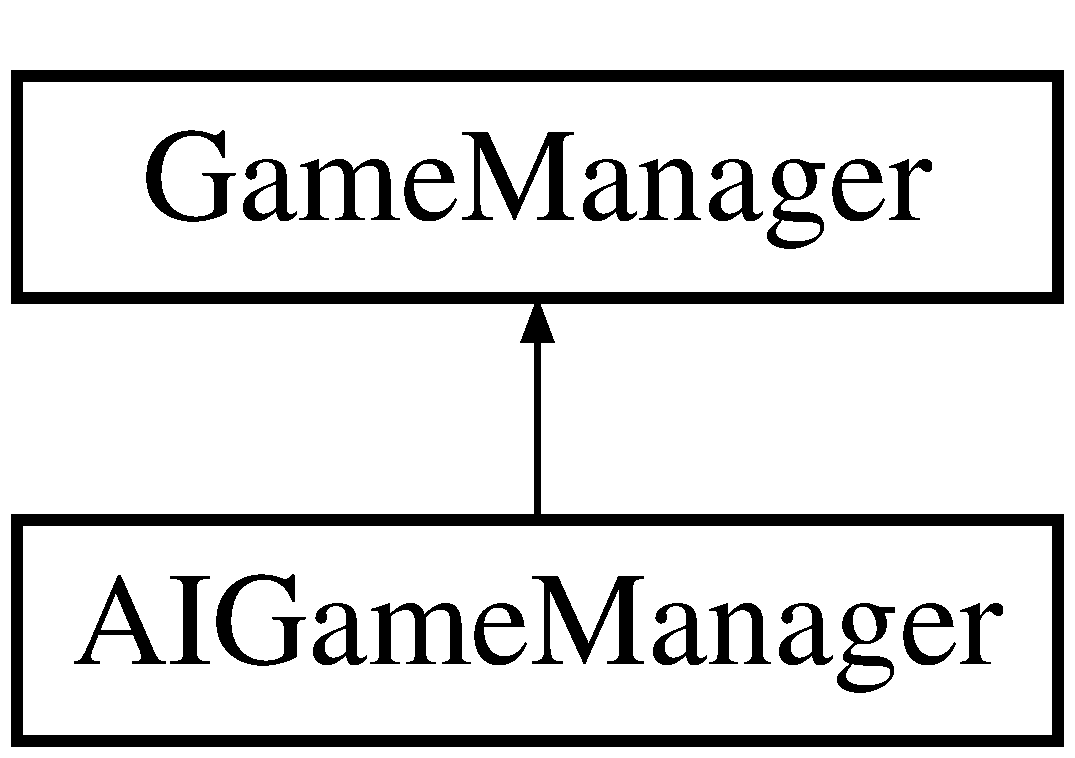
\includegraphics[height=2.000000cm]{classAIGameManager}
\end{center}
\end{figure}
\subsection*{\-Public \-Slots}
\begin{DoxyCompactItemize}
\item 
\hypertarget{classAIGameManager_a1dd46d003522dfad3572c0de445d1d20}{void \hyperlink{classAIGameManager_a1dd46d003522dfad3572c0de445d1d20}{mouse\-Press\-Event} (\-Q\-Mouse\-Event $\ast$event)}\label{classAIGameManager_a1dd46d003522dfad3572c0de445d1d20}

\begin{DoxyCompactList}\small\item\em drop coins and check finish game \end{DoxyCompactList}\end{DoxyCompactItemize}
\subsection*{\-Public \-Member \-Functions}
\begin{DoxyCompactItemize}
\item 
\hypertarget{classAIGameManager_a488945627859aff9401f1280f123bdc4}{{\bfseries \-A\-I\-Game\-Manager} (\-Q\-Widget $\ast$parent=0)}\label{classAIGameManager_a488945627859aff9401f1280f123bdc4}

\item 
\hypertarget{classAIGameManager_a91068d6c5076821cd5361efdbbc68fef}{void \hyperlink{classAIGameManager_a91068d6c5076821cd5361efdbbc68fef}{set\-Starting\-Player} (\hyperlink{structSettings}{\-Settings} settings)}\label{classAIGameManager_a91068d6c5076821cd5361efdbbc68fef}

\begin{DoxyCompactList}\small\item\em \-Sets the starting player depending wether ai should start. \end{DoxyCompactList}\end{DoxyCompactItemize}


\subsection{\-Detailed \-Description}
ai specific gamemanager 

\-A\-I specific gamemanger that handles the ai players turn

\begin{DoxyAuthor}{\-Author}
\-Roland \-Luckenthuber 

\-Denis \-Neuling 
\end{DoxyAuthor}


\-The documentation for this class was generated from the following files\-:\begin{DoxyCompactItemize}
\item 
aigamemanager.\-h\item 
aigamemanager.\-cpp\end{DoxyCompactItemize}

\hypertarget{structAnimation}{\section{\-Animation \-Struct \-Reference}
\label{structAnimation}\index{\-Animation@{\-Animation}}
}


handles animation state  




{\ttfamily \#include $<$animation.\-h$>$}

\subsection*{\-Public \-Attributes}
\begin{DoxyCompactItemize}
\item 
\hypertarget{structAnimation_ab7b2041b8fe676c3980eb27feb3c24d7}{bool {\bfseries active}}\label{structAnimation_ab7b2041b8fe676c3980eb27feb3c24d7}

\item 
\hypertarget{structAnimation_a0e5e8258f63ad3af3889c05dadbd50dd}{int {\bfseries current\-Y}}\label{structAnimation_a0e5e8258f63ad3af3889c05dadbd50dd}

\item 
\hypertarget{structAnimation_a270b071f76360d3a3d354fdc82034273}{int {\bfseries end\-Y}}\label{structAnimation_a270b071f76360d3a3d354fdc82034273}

\item 
\hypertarget{structAnimation_a4a79cc62a84e6f59fe7a9671c45e9afa}{int {\bfseries position\-X}}\label{structAnimation_a4a79cc62a84e6f59fe7a9671c45e9afa}

\item 
\hypertarget{structAnimation_ab9869e44134973b0d48506e8948cce40}{int {\bfseries start\-Y}}\label{structAnimation_ab9869e44134973b0d48506e8948cce40}

\item 
\hypertarget{structAnimation_ad8d4d4bba5b9accfba17cc9ecf5f3b50}{float {\bfseries time}}\label{structAnimation_ad8d4d4bba5b9accfba17cc9ecf5f3b50}

\item 
\hypertarget{structAnimation_a4d5850dde030ebc98d8f7a4427390ee4}{\-Coin {\bfseries player}}\label{structAnimation_a4d5850dde030ebc98d8f7a4427390ee4}

\end{DoxyCompactItemize}


\subsection{\-Detailed \-Description}
handles animation state 

\-Struct that handles animation state

\begin{DoxyAuthor}{\-Author}
\-Roland \-Luckenthuber 

\-Denis \-Neuling 
\end{DoxyAuthor}


\-The documentation for this struct was generated from the following file\-:\begin{DoxyCompactItemize}
\item 
animation.\-h\end{DoxyCompactItemize}

\hypertarget{classBoardColumn}{\section{\-Board\-Column \-Class \-Reference}
\label{classBoardColumn}\index{\-Board\-Column@{\-Board\-Column}}
}


column for the game board  




{\ttfamily \#include $<$boardcolumn.\-h$>$}

\subsection*{\-Public \-Member \-Functions}
\begin{DoxyCompactItemize}
\item 
\hypertarget{classBoardColumn_a8f088cd71325ffbdc839c101ca6a4fda}{{\bfseries \-Board\-Column} (int rows)}\label{classBoardColumn_a8f088cd71325ffbdc839c101ca6a4fda}

\item 
\hypertarget{classBoardColumn_adb1521008180835bd37572a1cda02ef8}{bool {\bfseries is\-Full} ()}\label{classBoardColumn_adb1521008180835bd37572a1cda02ef8}

\item 
\hypertarget{classBoardColumn_a09589c8bd6912dab8a7fb27500002553}{int {\bfseries get\-Current\-Amount\-Of\-Coins} ()}\label{classBoardColumn_a09589c8bd6912dab8a7fb27500002553}

\item 
\hypertarget{classBoardColumn_a060fd86473c5df6a98449e317bc2a364}{bool \hyperlink{classBoardColumn_a060fd86473c5df6a98449e317bc2a364}{add\-Coin} (\-Coin coin)}\label{classBoardColumn_a060fd86473c5df6a98449e317bc2a364}

\begin{DoxyCompactList}\small\item\em adds an coin to the boardcolumn \end{DoxyCompactList}\item 
\-Coin \hyperlink{classBoardColumn_a8b8107a2cb462ffd73d484b6e1d9b359}{get\-Coin} (int index)
\begin{DoxyCompactList}\small\item\em returns the coin at the specific index \end{DoxyCompactList}\item 
\hypertarget{classBoardColumn_ad4b43af3abf8de3332378529b7d5e743}{void \hyperlink{classBoardColumn_ad4b43af3abf8de3332378529b7d5e743}{remove\-Last\-Coin} ()}\label{classBoardColumn_ad4b43af3abf8de3332378529b7d5e743}

\begin{DoxyCompactList}\small\item\em removes the last added coin \end{DoxyCompactList}\item 
\hypertarget{classBoardColumn_a316e15e6e992dc3e0bba17289bad228a}{void \hyperlink{classBoardColumn_a316e15e6e992dc3e0bba17289bad228a}{clear} ()}\label{classBoardColumn_a316e15e6e992dc3e0bba17289bad228a}

\begin{DoxyCompactList}\small\item\em clears the boardcolumn \end{DoxyCompactList}\item 
\hypertarget{classBoardColumn_a8f088cd71325ffbdc839c101ca6a4fda}{{\bfseries \-Board\-Column} (int rows)}\label{classBoardColumn_a8f088cd71325ffbdc839c101ca6a4fda}

\item 
\hypertarget{classBoardColumn_adb1521008180835bd37572a1cda02ef8}{bool {\bfseries is\-Full} ()}\label{classBoardColumn_adb1521008180835bd37572a1cda02ef8}

\item 
\hypertarget{classBoardColumn_a09589c8bd6912dab8a7fb27500002553}{int {\bfseries get\-Current\-Amount\-Of\-Coins} ()}\label{classBoardColumn_a09589c8bd6912dab8a7fb27500002553}

\item 
\hypertarget{classBoardColumn_a060fd86473c5df6a98449e317bc2a364}{bool {\bfseries add\-Coin} (\-Coin coin)}\label{classBoardColumn_a060fd86473c5df6a98449e317bc2a364}

\item 
\hypertarget{classBoardColumn_a8b8107a2cb462ffd73d484b6e1d9b359}{\-Coin {\bfseries get\-Coin} (int index)}\label{classBoardColumn_a8b8107a2cb462ffd73d484b6e1d9b359}

\end{DoxyCompactItemize}


\subsection{\-Detailed \-Description}
column for the game board 

column placed at the the game board

\begin{DoxyAuthor}{\-Author}
\-Roland \-Luckenthuber 

\-Denis \-Neuling 
\end{DoxyAuthor}


\subsection{\-Member \-Function \-Documentation}
\hypertarget{classBoardColumn_a8b8107a2cb462ffd73d484b6e1d9b359}{\index{\-Board\-Column@{\-Board\-Column}!get\-Coin@{get\-Coin}}
\index{get\-Coin@{get\-Coin}!BoardColumn@{\-Board\-Column}}
\subsubsection[{get\-Coin}]{\setlength{\rightskip}{0pt plus 5cm}\-Coin {\bf \-Board\-Column\-::get\-Coin} (
\begin{DoxyParamCaption}
\item[{int}]{index}
\end{DoxyParamCaption}
)\hspace{0.3cm}{\ttfamily  \mbox{[}inline\mbox{]}}}}\label{classBoardColumn_a8b8107a2cb462ffd73d484b6e1d9b359}


returns the coin at the specific index 


\begin{DoxyParams}{\-Parameters}
{\em index} & the index of the coin \\
\hline
\end{DoxyParams}


\-The documentation for this class was generated from the following files\-:\begin{DoxyCompactItemize}
\item 
boardcolumn.\-h\item 
column.\-h\item 
column.\-cpp\end{DoxyCompactItemize}

\hypertarget{classConnectFourObject}{\section{\-Connect\-Four\-Object \-Class \-Reference}
\label{classConnectFourObject}\index{\-Connect\-Four\-Object@{\-Connect\-Four\-Object}}
}


base class for every connect four related class  




{\ttfamily \#include $<$connectfourobject.\-h$>$}

\-Inheritance diagram for \-Connect\-Four\-Object\-:\begin{figure}[H]
\begin{center}
\leavevmode
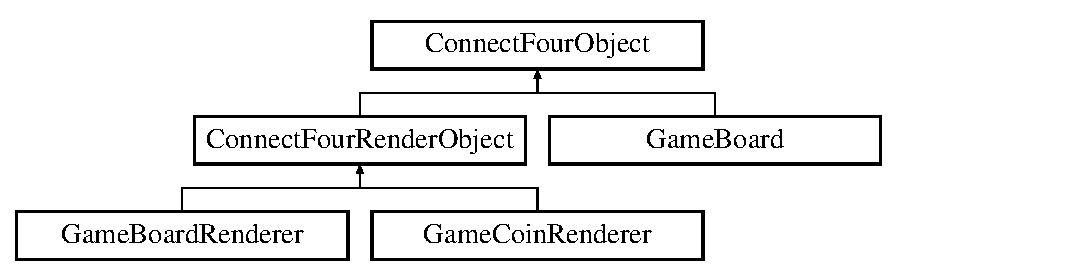
\includegraphics[height=3.000000cm]{classConnectFourObject}
\end{center}
\end{figure}
\subsection*{\-Public \-Member \-Functions}
\begin{DoxyCompactItemize}
\item 
\hypertarget{classConnectFourObject_a6dabab64cdbd0b264aebf42435dd901b}{{\bfseries \-Connect\-Four\-Object} (int width, int height)}\label{classConnectFourObject_a6dabab64cdbd0b264aebf42435dd901b}

\end{DoxyCompactItemize}
\subsection*{\-Protected \-Attributes}
\begin{DoxyCompactItemize}
\item 
\hypertarget{classConnectFourObject_ae6e240f90182a3ff58790a1307ccd1b1}{int {\bfseries m\-\_\-\-Rows}}\label{classConnectFourObject_ae6e240f90182a3ff58790a1307ccd1b1}

\item 
\hypertarget{classConnectFourObject_a6a2622a917669b269f88af84f25425eb}{int {\bfseries m\-\_\-\-Columns}}\label{classConnectFourObject_a6a2622a917669b269f88af84f25425eb}

\end{DoxyCompactItemize}


\subsection{\-Detailed \-Description}
base class for every connect four related class 

base class for every connect four related class

\begin{DoxyAuthor}{\-Author}
\-Roland \-Luckenthuber 

\-Denis \-Neuling 
\end{DoxyAuthor}


\-The documentation for this class was generated from the following file\-:\begin{DoxyCompactItemize}
\item 
connectfourobject.\-h\end{DoxyCompactItemize}

\hypertarget{classConnectFourRenderObject}{\section{\-Connect\-Four\-Render\-Object \-Class \-Reference}
\label{classConnectFourRenderObject}\index{\-Connect\-Four\-Render\-Object@{\-Connect\-Four\-Render\-Object}}
}


base class for each renderable connect four object  




{\ttfamily \#include $<$connectfourrenderobject.\-h$>$}

\-Inheritance diagram for \-Connect\-Four\-Render\-Object\-:\begin{figure}[H]
\begin{center}
\leavevmode
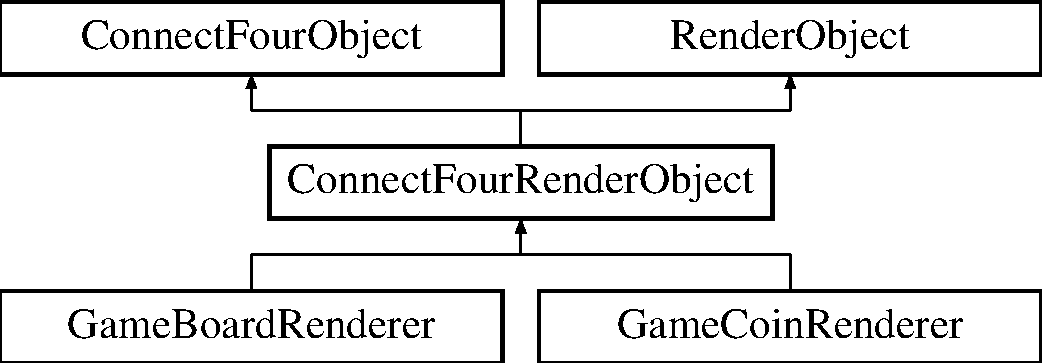
\includegraphics[height=3.000000cm]{classConnectFourRenderObject}
\end{center}
\end{figure}
\subsection*{\-Public \-Member \-Functions}
\begin{DoxyCompactItemize}
\item 
\hypertarget{classConnectFourRenderObject_ab89a0ead57bcac10a73a2e01969e86c6}{{\bfseries \-Connect\-Four\-Render\-Object} (int width, int height, float cell\-Size)}\label{classConnectFourRenderObject_ab89a0ead57bcac10a73a2e01969e86c6}

\item 
\hypertarget{classConnectFourRenderObject_a9b29bbc57d9985db1075a1b147b15801}{virtual void {\bfseries resize} (int width, int height)}\label{classConnectFourRenderObject_a9b29bbc57d9985db1075a1b147b15801}

\end{DoxyCompactItemize}
\subsection*{\-Protected \-Attributes}
\begin{DoxyCompactItemize}
\item 
\hypertarget{classConnectFourRenderObject_a507319d76cc95bd30ca5a8e4e5e4e5c6}{float {\bfseries m\-\_\-\-Cell\-Size}}\label{classConnectFourRenderObject_a507319d76cc95bd30ca5a8e4e5e4e5c6}

\item 
\hypertarget{classConnectFourRenderObject_afa3cd5255b779a30c8f8a3615f5a6c14}{float {\bfseries m\-\_\-\-Coin\-Radius}}\label{classConnectFourRenderObject_afa3cd5255b779a30c8f8a3615f5a6c14}

\item 
\hypertarget{classConnectFourRenderObject_aa864124c16d148218a340af0340d6ddf}{float {\bfseries m\-\_\-\-Scale}}\label{classConnectFourRenderObject_aa864124c16d148218a340af0340d6ddf}

\end{DoxyCompactItemize}


\subsection{\-Detailed \-Description}
base class for each renderable connect four object 

base class for each renderable connect four object

\begin{DoxyAuthor}{\-Author}
\-Roland \-Luckenthuber 

\-Denis \-Neuling 
\end{DoxyAuthor}


\-The documentation for this class was generated from the following file\-:\begin{DoxyCompactItemize}
\item 
connectfourrenderobject.\-h\end{DoxyCompactItemize}

\hypertarget{structGame}{\section{\-Game \-Struct \-Reference}
\label{structGame}\index{\-Game@{\-Game}}
}


data holder for game results  




{\ttfamily \#include $<$game.\-h$>$}

\subsection*{\-Public \-Member \-Functions}
\begin{DoxyCompactItemize}
\item 
\hypertarget{structGame_a044fef9d8dfbbece3bafa8762991d50a}{{\bfseries \-Game} (\-Result result)}\label{structGame_a044fef9d8dfbbece3bafa8762991d50a}

\item 
\hypertarget{structGame_a5e9801592737721fdaecfb2e7b00cc13}{{\bfseries \-Game} (\-Result result, \hyperlink{classPlayer}{\-Player} winner, \hyperlink{classPlayer}{\-Player} loser)}\label{structGame_a5e9801592737721fdaecfb2e7b00cc13}

\item 
\hypertarget{structGame_a0aa609437b4295dba61e18b7e01cc2a7}{\-Q\-String {\bfseries to\-String} ()}\label{structGame_a0aa609437b4295dba61e18b7e01cc2a7}

\end{DoxyCompactItemize}
\subsection*{\-Public \-Attributes}
\begin{DoxyCompactItemize}
\item 
\hypertarget{structGame_a9649ed9f4a7e37744396a793d345a222}{\-Result {\bfseries result}}\label{structGame_a9649ed9f4a7e37744396a793d345a222}

\item 
\hypertarget{structGame_a590df81200f797fd5bef8c5968a2ea1b}{\hyperlink{classPlayer}{\-Player} {\bfseries winner}}\label{structGame_a590df81200f797fd5bef8c5968a2ea1b}

\item 
\hypertarget{structGame_a151b35fd4e46d2152eb7e5d196e0b4de}{\hyperlink{classPlayer}{\-Player} {\bfseries loser}}\label{structGame_a151b35fd4e46d2152eb7e5d196e0b4de}

\end{DoxyCompactItemize}


\subsection{\-Detailed \-Description}
data holder for game results 

data holder for game results

\begin{DoxyAuthor}{\-Author}
\-Roland \-Luckenthuber 

\-Denis \-Neuling 
\end{DoxyAuthor}


\-The documentation for this struct was generated from the following file\-:\begin{DoxyCompactItemize}
\item 
game.\-h\end{DoxyCompactItemize}

\hypertarget{classGameBoard}{\section{\-Game\-Board \-Class \-Reference}
\label{classGameBoard}\index{\-Game\-Board@{\-Game\-Board}}
}


game board class representing game board  




{\ttfamily \#include $<$gameboard.\-h$>$}

\-Inheritance diagram for \-Game\-Board\-:\begin{figure}[H]
\begin{center}
\leavevmode
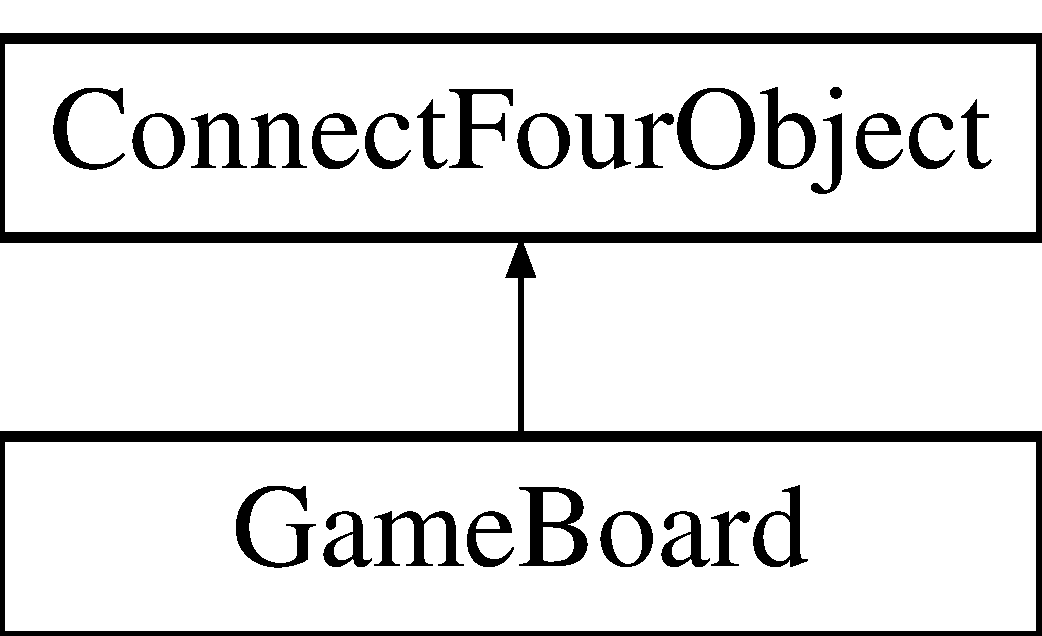
\includegraphics[height=2.000000cm]{classGameBoard}
\end{center}
\end{figure}
\subsection*{\-Public \-Member \-Functions}
\begin{DoxyCompactItemize}
\item 
\hypertarget{classGameBoard_ae9975214e1b9b33c8d796937aa42520e}{{\bfseries \-Game\-Board} (int rows, int columns, \-Q\-Object $\ast$parent=0)}\label{classGameBoard_ae9975214e1b9b33c8d796937aa42520e}

\item 
\hypertarget{classGameBoard_ac3f19f16873e19e03d56b06ced39792c}{{\bfseries \-Game\-Board} (const \hyperlink{classGameBoard}{\-Game\-Board} \&other)}\label{classGameBoard_ac3f19f16873e19e03d56b06ced39792c}

\item 
bool \hyperlink{classGameBoard_a706ae720beb9de8147298676dc75283c}{add\-Coin} (int column, \-Coin coin)
\begin{DoxyCompactList}\small\item\em add coin to the game board at the specific column \end{DoxyCompactList}\item 
\hypertarget{classGameBoard_a99daa5b67393b74abddfd293b17a2acb}{void {\bfseries remove\-Coin} (int column)}\label{classGameBoard_a99daa5b67393b74abddfd293b17a2acb}

\item 
\hypertarget{classGameBoard_a72290b30d47b27d1a929150cd9d16305}{\-Result \hyperlink{classGameBoard_a72290b30d47b27d1a929150cd9d16305}{check\-Game\-Conditions} ()}\label{classGameBoard_a72290b30d47b27d1a929150cd9d16305}

\begin{DoxyCompactList}\small\item\em check if the game is over \end{DoxyCompactList}\item 
\hypertarget{classGameBoard_ad2c44e434b52ccb41d4b272b498cbbac}{std\-::vector$<$ int $>$ \hyperlink{classGameBoard_ad2c44e434b52ccb41d4b272b498cbbac}{get\-Available\-Moves} ()}\label{classGameBoard_ad2c44e434b52ccb41d4b272b498cbbac}

\begin{DoxyCompactList}\small\item\em returns list of available columns \end{DoxyCompactList}\item 
\hypertarget{classGameBoard_ae90c2043ae979dc35dea08113bac278a}{std\-::vector$<$ std\-::shared\-\_\-ptr\*
$<$ \hyperlink{classBoardColumn}{\-Board\-Column} $>$ $>$ {\bfseries get\-Current\-Board} ()}\label{classGameBoard_ae90c2043ae979dc35dea08113bac278a}

\item 
\hypertarget{classGameBoard_ad533f495fa4f39c15e1164a1a5bb702e}{\-Q\-String {\bfseries serialize} ()}\label{classGameBoard_ad533f495fa4f39c15e1164a1a5bb702e}

\item 
\hypertarget{classGameBoard_abfd027ca1bf36698290855faff44d1a3}{void {\bfseries deserialize} (\-Q\-String board)}\label{classGameBoard_abfd027ca1bf36698290855faff44d1a3}

\end{DoxyCompactItemize}
\subsection*{\-Protected \-Member \-Functions}
\begin{DoxyCompactItemize}
\item 
\hypertarget{classGameBoard_a9d39bb64647af701a265251624287807}{bool {\bfseries check\-Draw\-Conditions} ()}\label{classGameBoard_a9d39bb64647af701a265251624287807}

\item 
\hypertarget{classGameBoard_a2ac14f3ff1d653e086136792fe0933d6}{\-Coin {\bfseries check\-Win\-Conditions} ()}\label{classGameBoard_a2ac14f3ff1d653e086136792fe0933d6}

\item 
\hypertarget{classGameBoard_a15b19b2ec1e4c63b47e113aba42d3ae3}{\-Coin {\bfseries get\-Coin} (int column, int row)}\label{classGameBoard_a15b19b2ec1e4c63b47e113aba42d3ae3}

\item 
\hypertarget{classGameBoard_ae43c300f4bc9df8a8d65231f96d335dd}{bool {\bfseries is\-Coin\-Valid\-At} (int column, int row)}\label{classGameBoard_ae43c300f4bc9df8a8d65231f96d335dd}

\end{DoxyCompactItemize}
\subsection*{\-Protected \-Attributes}
\begin{DoxyCompactItemize}
\item 
\hypertarget{classGameBoard_a62a11c93b4a0af85d3613351ac323485}{std\-::vector$<$ std\-::shared\-\_\-ptr\*
$<$ \hyperlink{classBoardColumn}{\-Board\-Column} $>$ $>$ {\bfseries m\-\_\-p\-Game\-Board}}\label{classGameBoard_a62a11c93b4a0af85d3613351ac323485}

\end{DoxyCompactItemize}


\subsection{\-Detailed \-Description}
game board class representing game board 

game board splitted up into columns and rows handling coins

\begin{DoxyAuthor}{\-Author}
\-Roland \-Luckenthuber 

\-Denis \-Neuling 
\end{DoxyAuthor}


\subsection{\-Member \-Function \-Documentation}
\hypertarget{classGameBoard_a706ae720beb9de8147298676dc75283c}{\index{\-Game\-Board@{\-Game\-Board}!add\-Coin@{add\-Coin}}
\index{add\-Coin@{add\-Coin}!GameBoard@{\-Game\-Board}}
\subsubsection[{add\-Coin}]{\setlength{\rightskip}{0pt plus 5cm}bool {\bf \-Game\-Board\-::add\-Coin} (
\begin{DoxyParamCaption}
\item[{int}]{column, }
\item[{\-Coin}]{coin}
\end{DoxyParamCaption}
)}}\label{classGameBoard_a706ae720beb9de8147298676dc75283c}


add coin to the game board at the specific column 


\begin{DoxyParams}{\-Parameters}
{\em column} & the column where the coin should be added \\
\hline
{\em the} & coin to add \\
\hline
\end{DoxyParams}


\-The documentation for this class was generated from the following files\-:\begin{DoxyCompactItemize}
\item 
gameboard.\-h\item 
gameboard.\-cpp\end{DoxyCompactItemize}

\hypertarget{classGameBoardRenderer}{\section{\-Game\-Board\-Renderer \-Class \-Reference}
\label{classGameBoardRenderer}\index{\-Game\-Board\-Renderer@{\-Game\-Board\-Renderer}}
}


\-Class that is responsible for rendering the gameboard.  




{\ttfamily \#include $<$gameboardrenderer.\-h$>$}

\-Inheritance diagram for \-Game\-Board\-Renderer\-:\begin{figure}[H]
\begin{center}
\leavevmode
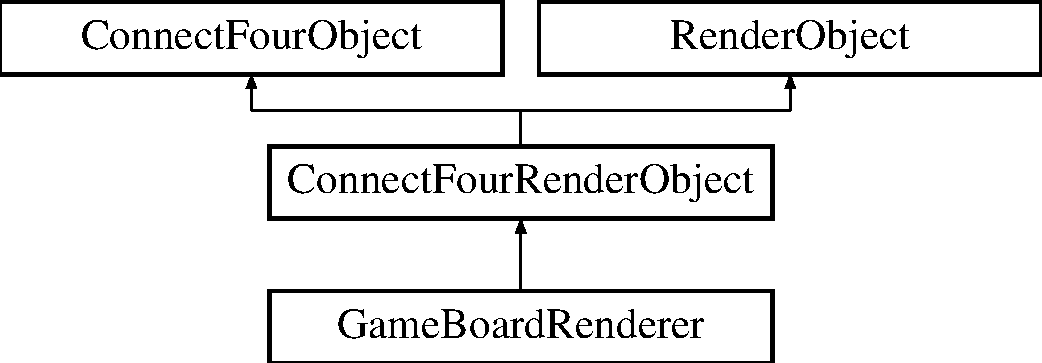
\includegraphics[height=3.000000cm]{classGameBoardRenderer}
\end{center}
\end{figure}
\subsection*{\-Public \-Member \-Functions}
\begin{DoxyCompactItemize}
\item 
\hypertarget{classGameBoardRenderer_a7ca6fb62b4ed41b70d7e8883e31d20a2}{{\bfseries \-Game\-Board\-Renderer} (int width, int height, float cell\-Size)}\label{classGameBoardRenderer_a7ca6fb62b4ed41b70d7e8883e31d20a2}

\item 
\hypertarget{classGameBoardRenderer_a5b45052cf71976461b07721195dd5dbe}{void {\bfseries init} ()}\label{classGameBoardRenderer_a5b45052cf71976461b07721195dd5dbe}

\item 
\hypertarget{classGameBoardRenderer_a9daf708f14cd6accf1e2f4cc54bb7d56}{void {\bfseries draw} ()}\label{classGameBoardRenderer_a9daf708f14cd6accf1e2f4cc54bb7d56}

\item 
\hypertarget{classGameBoardRenderer_a816b3c402bf466641681ed67cefe1041}{int {\bfseries calculate\-And\-Set\-Column\-From\-Mouse\-Point} (\-Q\-Point point)}\label{classGameBoardRenderer_a816b3c402bf466641681ed67cefe1041}

\item 
\hypertarget{classGameBoardRenderer_a5678cf7626743de3844406465ca2bf6f}{void {\bfseries set\-Current\-Active\-Player} (\-Coin player)}\label{classGameBoardRenderer_a5678cf7626743de3844406465ca2bf6f}

\end{DoxyCompactItemize}


\subsection{\-Detailed \-Description}
\-Class that is responsible for rendering the gameboard. 

renders the game board grid

\begin{DoxyAuthor}{\-Author}
\-Roland \-Luckenthuber 

\-Denis \-Neuling 
\end{DoxyAuthor}


\-The documentation for this class was generated from the following files\-:\begin{DoxyCompactItemize}
\item 
gameboardrenderer.\-h\item 
gameboardrenderer.\-cpp\end{DoxyCompactItemize}

\hypertarget{classGameClient}{\section{\-Game\-Client \-Class \-Reference}
\label{classGameClient}\index{\-Game\-Client@{\-Game\-Client}}
}


\-Class that is responsible for opening a tcp socket connection to the host.  




{\ttfamily \#include $<$gameclient.\-h$>$}

\-Inheritance diagram for \-Game\-Client\-:\begin{figure}[H]
\begin{center}
\leavevmode
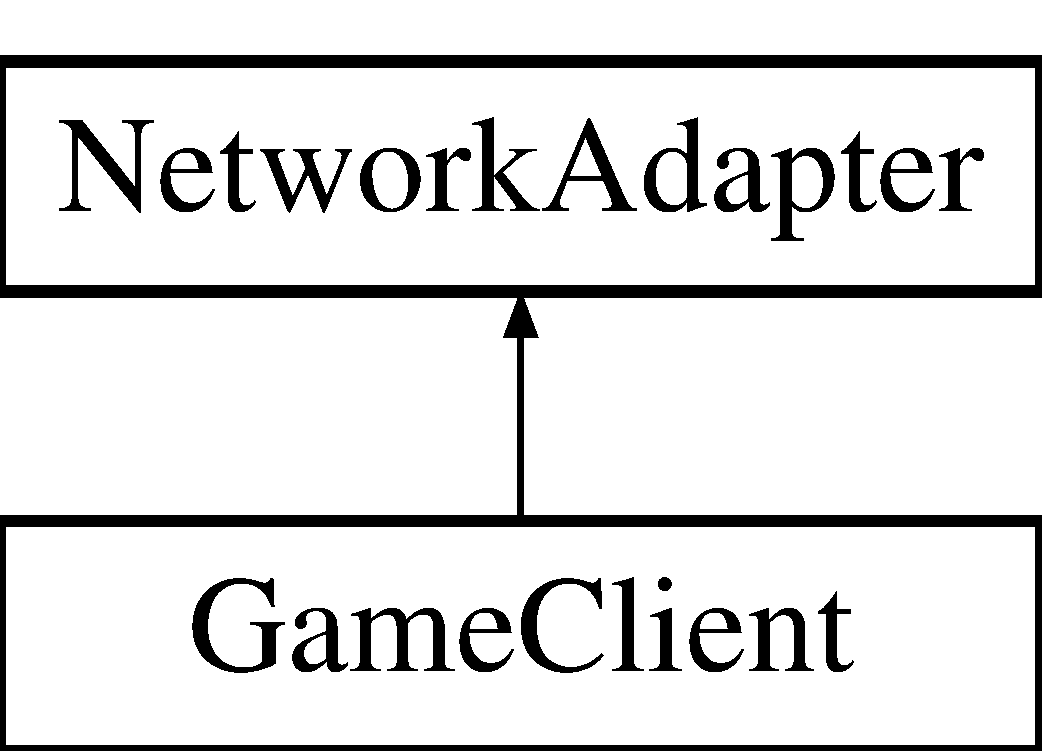
\includegraphics[height=2.000000cm]{classGameClient}
\end{center}
\end{figure}
\subsection*{\-Public \-Slots}
\begin{DoxyCompactItemize}
\item 
\hypertarget{classGameClient_aac63bd682b0cfde980b042bf8145e883}{void \hyperlink{classGameClient_aac63bd682b0cfde980b042bf8145e883}{connected} ()}\label{classGameClient_aac63bd682b0cfde980b042bf8145e883}

\begin{DoxyCompactList}\small\item\em called when connected to the server \end{DoxyCompactList}\item 
\hypertarget{classGameClient_a5457bdb6b9a17067bbb67a2498ee395d}{void \hyperlink{classGameClient_a5457bdb6b9a17067bbb67a2498ee395d}{read\-Ready} ()}\label{classGameClient_a5457bdb6b9a17067bbb67a2498ee395d}

\begin{DoxyCompactList}\small\item\em called when new data is available from the client \end{DoxyCompactList}\end{DoxyCompactItemize}
\subsection*{\-Public \-Member \-Functions}
\begin{DoxyCompactItemize}
\item 
\hypertarget{classGameClient_a6c6faf6d8e0524f9b75041b3eaeb718d}{{\bfseries \-Game\-Client} (\-Q\-String ip\-Address, \-Q\-Object $\ast$parent=0)}\label{classGameClient_a6c6faf6d8e0524f9b75041b3eaeb718d}

\item 
\hypertarget{classGameClient_a96c861f5f70e645a28cf6e7a042dfc9f}{void {\bfseries init} ()}\label{classGameClient_a96c861f5f70e645a28cf6e7a042dfc9f}

\item 
\hypertarget{classGameClient_ad6130cb3cddc509730c948e0177c1be2}{void {\bfseries send} (\-Q\-String data)}\label{classGameClient_ad6130cb3cddc509730c948e0177c1be2}

\end{DoxyCompactItemize}


\subsection{\-Detailed \-Description}
\-Class that is responsible for opening a tcp socket connection to the host. 

\-Class handles a tcp socket connection to the host

\begin{DoxyAuthor}{\-Author}
\-Roland \-Luckenthuber 

\-Denis \-Neuling 
\end{DoxyAuthor}


\-The documentation for this class was generated from the following files\-:\begin{DoxyCompactItemize}
\item 
gameclient.\-h\item 
gameclient.\-cpp\end{DoxyCompactItemize}

\hypertarget{classGameCoinRenderer}{\section{\-Game\-Coin\-Renderer \-Class \-Reference}
\label{classGameCoinRenderer}\index{\-Game\-Coin\-Renderer@{\-Game\-Coin\-Renderer}}
}


\-Class that is responsible for rendering the coins added to the board.  




{\ttfamily \#include $<$gamecoinrenderer.\-h$>$}

\-Inheritance diagram for \-Game\-Coin\-Renderer\-:\begin{figure}[H]
\begin{center}
\leavevmode
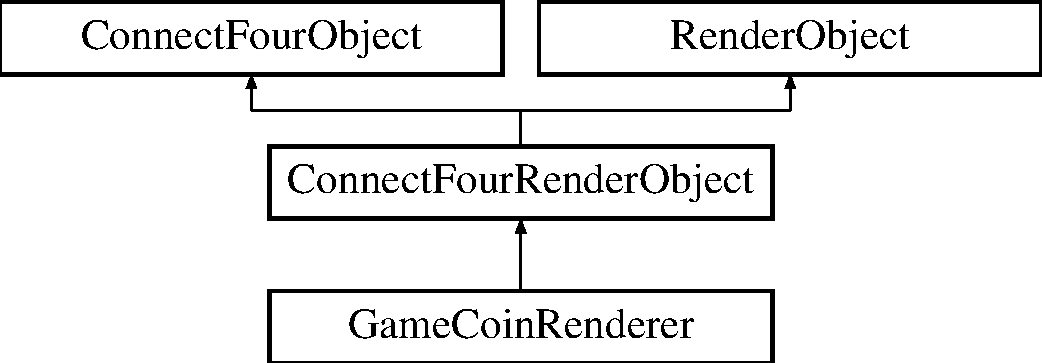
\includegraphics[height=3.000000cm]{classGameCoinRenderer}
\end{center}
\end{figure}
\subsection*{\-Public \-Member \-Functions}
\begin{DoxyCompactItemize}
\item 
\hypertarget{classGameCoinRenderer_a74dd1dd742641b6585df5fe24d4c4e62}{{\bfseries \-Game\-Coin\-Renderer} (int width, int height, float cell\-Size)}\label{classGameCoinRenderer_a74dd1dd742641b6585df5fe24d4c4e62}

\item 
\hypertarget{classGameCoinRenderer_a2b1b51d93a38675ee1f30fc6cacbaccd}{virtual void \hyperlink{classGameCoinRenderer_a2b1b51d93a38675ee1f30fc6cacbaccd}{draw} ()}\label{classGameCoinRenderer_a2b1b51d93a38675ee1f30fc6cacbaccd}

\begin{DoxyCompactList}\small\item\em renders the board \end{DoxyCompactList}\item 
\hypertarget{classGameCoinRenderer_a88ecbeec05a81381ee676463fe2aac53}{void \hyperlink{classGameCoinRenderer_a88ecbeec05a81381ee676463fe2aac53}{update\-Game\-Coins} (int column, \-Coin coin)}\label{classGameCoinRenderer_a88ecbeec05a81381ee676463fe2aac53}

\begin{DoxyCompactList}\small\item\em adds coins to the board \end{DoxyCompactList}\item 
\hypertarget{classGameCoinRenderer_a20a3e2499f4f1656a3e1012ef34e7e89}{void \hyperlink{classGameCoinRenderer_a20a3e2499f4f1656a3e1012ef34e7e89}{set\-Game\-Board} (std\-::vector$<$ std\-::shared\-\_\-ptr$<$ \hyperlink{classBoardColumn}{\-Board\-Column} $>$ $>$ board)}\label{classGameCoinRenderer_a20a3e2499f4f1656a3e1012ef34e7e89}

\begin{DoxyCompactList}\small\item\em updates the whole board \end{DoxyCompactList}\end{DoxyCompactItemize}


\subsection{\-Detailed \-Description}
\-Class that is responsible for rendering the coins added to the board. 

\-Class that is responsible for rendering the coins added to the board

\begin{DoxyAuthor}{\-Author}
\-Roland \-Luckenthuber 

\-Denis \-Neuling 
\end{DoxyAuthor}


\-The documentation for this class was generated from the following files\-:\begin{DoxyCompactItemize}
\item 
gamecoinrenderer.\-h\item 
gamecoinrenderer.\-cpp\end{DoxyCompactItemize}

\hypertarget{classGameDatabase}{\section{\-Game\-Database \-Class \-Reference}
\label{classGameDatabase}\index{\-Game\-Database@{\-Game\-Database}}
}


singleton class that manages the game result database  




{\ttfamily \#include $<$gamedatabase.\-h$>$}

\subsection*{\-Public \-Member \-Functions}
\begin{DoxyCompactItemize}
\item 
void \hyperlink{classGameDatabase_aa2e298187a235ff09b53444b65ef806c}{add\-Game} (\hyperlink{structGame}{\-Game} game)
\begin{DoxyCompactList}\small\item\em \-Adds a game to the database. \end{DoxyCompactList}\item 
\hypertarget{classGameDatabase_a11efba57db9c500a523ce51cd156dd35}{\-Q\-String\-List {\bfseries get\-Games} ()}\label{classGameDatabase_a11efba57db9c500a523ce51cd156dd35}

\end{DoxyCompactItemize}
\subsection*{\-Static \-Public \-Member \-Functions}
\begin{DoxyCompactItemize}
\item 
\hypertarget{classGameDatabase_a216477b314b74b86d42c943b359ac33a}{static \hyperlink{classGameDatabase}{\-Game\-Database} \& {\bfseries get\-Instance} ()}\label{classGameDatabase_a216477b314b74b86d42c943b359ac33a}

\end{DoxyCompactItemize}


\subsection{\-Detailed \-Description}
singleton class that manages the game result database 

singleton class that manages the game result database

\begin{DoxyAuthor}{\-Author}
\-Roland \-Luckenthuber 

\-Denis \-Neuling 
\end{DoxyAuthor}


\subsection{\-Member \-Function \-Documentation}
\hypertarget{classGameDatabase_aa2e298187a235ff09b53444b65ef806c}{\index{\-Game\-Database@{\-Game\-Database}!add\-Game@{add\-Game}}
\index{add\-Game@{add\-Game}!GameDatabase@{\-Game\-Database}}
\subsubsection[{add\-Game}]{\setlength{\rightskip}{0pt plus 5cm}void {\bf \-Game\-Database\-::add\-Game} (
\begin{DoxyParamCaption}
\item[{{\bf \-Game}}]{game}
\end{DoxyParamCaption}
)}}\label{classGameDatabase_aa2e298187a235ff09b53444b65ef806c}


\-Adds a game to the database. 


\begin{DoxyParams}{\-Parameters}
{\em the} & game to add \\
\hline
\end{DoxyParams}


\-The documentation for this class was generated from the following files\-:\begin{DoxyCompactItemize}
\item 
gamedatabase.\-h\item 
gamedatabase.\-cpp\end{DoxyCompactItemize}

\hypertarget{classGameManager}{\section{\-Game\-Manager \-Class \-Reference}
\label{classGameManager}\index{\-Game\-Manager@{\-Game\-Manager}}
}


\-Class that handles game states and instanciates renderer and board.  




{\ttfamily \#include $<$gamemanager.\-h$>$}

\-Inheritance diagram for \-Game\-Manager\-:\begin{figure}[H]
\begin{center}
\leavevmode
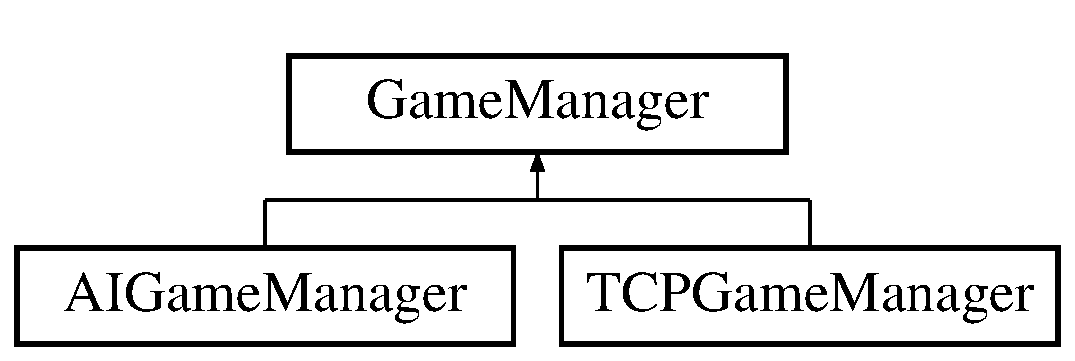
\includegraphics[height=2.000000cm]{classGameManager}
\end{center}
\end{figure}
\subsection*{\-Public \-Slots}
\begin{DoxyCompactItemize}
\item 
\hypertarget{classGameManager_a55876082b15630acf8109b5f0a33e6bd}{void {\bfseries game\-End} ()}\label{classGameManager_a55876082b15630acf8109b5f0a33e6bd}

\item 
\hypertarget{classGameManager_a7ecc3a14cd9e92f50729b37d1364953f}{void \hyperlink{classGameManager_a7ecc3a14cd9e92f50729b37d1364953f}{update} ()}\label{classGameManager_a7ecc3a14cd9e92f50729b37d1364953f}

\begin{DoxyCompactList}\small\item\em poll mouse position and update states \end{DoxyCompactList}\item 
\hypertarget{classGameManager_ac15bf5701604781f66047dc8c94f70a7}{void \hyperlink{classGameManager_ac15bf5701604781f66047dc8c94f70a7}{mouse\-Press\-Event} (\-Q\-Mouse\-Event $\ast$event)}\label{classGameManager_ac15bf5701604781f66047dc8c94f70a7}

\begin{DoxyCompactList}\small\item\em drop coins and check finish game \end{DoxyCompactList}\item 
\hypertarget{classGameManager_a452f27d846213676394663c8d223983d}{void {\bfseries save\-Game} ()}\label{classGameManager_a452f27d846213676394663c8d223983d}

\item 
\hypertarget{classGameManager_ad7e262dd756247130c085ead21b34d87}{void \hyperlink{classGameManager_ad7e262dd756247130c085ead21b34d87}{load\-Game} (\-Q\-String game\-Board)}\label{classGameManager_ad7e262dd756247130c085ead21b34d87}

\begin{DoxyCompactList}\small\item\em also handles start game \end{DoxyCompactList}\item 
\hypertarget{classGameManager_af49538ffbacf3ed465fe23191f0a7378}{void {\bfseries switch\-Player} ()}\label{classGameManager_af49538ffbacf3ed465fe23191f0a7378}

\item 
\hypertarget{classGameManager_aef672bf56ae84eb10a65bf227e487717}{\hyperlink{classPlayer}{\-Player} {\bfseries get\-Current\-Active\-Player} ()}\label{classGameManager_aef672bf56ae84eb10a65bf227e487717}

\item 
\hypertarget{classGameManager_a875582122292a52ffcae786a46490f89}{\hyperlink{classPlayer}{\-Player} {\bfseries get\-Current\-Inactive\-Player} ()}\label{classGameManager_a875582122292a52ffcae786a46490f89}

\end{DoxyCompactItemize}
\subsection*{\-Signals}
\begin{DoxyCompactItemize}
\item 
\hypertarget{classGameManager_ae63cd6e5b6b2458d5260d421433aa43c}{void {\bfseries game\-Started} ()}\label{classGameManager_ae63cd6e5b6b2458d5260d421433aa43c}

\end{DoxyCompactItemize}
\subsection*{\-Public \-Member \-Functions}
\begin{DoxyCompactItemize}
\item 
\hypertarget{classGameManager_a22f8d699d465b1246ed1ca95cb5e8126}{{\bfseries \-Game\-Manager} (\-Q\-Widget $\ast$parent=0)}\label{classGameManager_a22f8d699d465b1246ed1ca95cb5e8126}

\item 
\hypertarget{classGameManager_a4acbc34fa6c280d0f6d48ff867626ce2}{virtual void \hyperlink{classGameManager_a4acbc34fa6c280d0f6d48ff867626ce2}{start\-Game} (\hyperlink{structSettings}{\-Settings} settings)}\label{classGameManager_a4acbc34fa6c280d0f6d48ff867626ce2}

\begin{DoxyCompactList}\small\item\em instanciates renderer and gameboard \end{DoxyCompactList}\item 
\hypertarget{classGameManager_a6ec9d87c1a6366be0f5b2191b798a679}{virtual void \hyperlink{classGameManager_a6ec9d87c1a6366be0f5b2191b798a679}{set\-Starting\-Player} (\hyperlink{structSettings}{\-Settings} settings, \-Coin player=\-R\-E\-D)}\label{classGameManager_a6ec9d87c1a6366be0f5b2191b798a679}

\begin{DoxyCompactList}\small\item\em used for diffent game managers to handle starting player \end{DoxyCompactList}\item 
\hypertarget{classGameManager_afc363c6765b4fdf990f75bd5978a9dbb}{void {\bfseries finish\-Game} (\hyperlink{structGame}{\-Game} game)}\label{classGameManager_afc363c6765b4fdf990f75bd5978a9dbb}

\end{DoxyCompactItemize}
\subsection*{\-Protected \-Member \-Functions}
\begin{DoxyCompactItemize}
\item 
\hypertarget{classGameManager_a4d65975808a9ddce05814b0708b11268}{void {\bfseries check\-And\-Handle\-Win} (int column)}\label{classGameManager_a4d65975808a9ddce05814b0708b11268}

\end{DoxyCompactItemize}
\subsection*{\-Protected \-Attributes}
\begin{DoxyCompactItemize}
\item 
\hypertarget{classGameManager_aee76ef2de914b2c0934c5b3264426edb}{\-Q\-H\-Box\-Layout $\ast$ {\bfseries m\-\_\-p\-Main\-Layout}}\label{classGameManager_aee76ef2de914b2c0934c5b3264426edb}

\item 
\hypertarget{classGameManager_af15f419d79f18cf1bfb846633fa60ea6}{\hyperlink{classGameRenderer}{\-Game\-Renderer} $\ast$ {\bfseries m\-\_\-p\-Renderer}}\label{classGameManager_af15f419d79f18cf1bfb846633fa60ea6}

\item 
\hypertarget{classGameManager_af8185baa9bd771d56187bfe21a35bcca}{\hyperlink{classGameBoard}{\-Game\-Board} $\ast$ {\bfseries m\-\_\-p\-Game\-Board}}\label{classGameManager_af8185baa9bd771d56187bfe21a35bcca}

\item 
\hypertarget{classGameManager_a8f611fd41149c74160bf1314d3c8ce09}{\hyperlink{classGameOverScreen}{\-Game\-Over\-Screen} $\ast$ {\bfseries m\-\_\-p\-Game\-Over\-Screen}}\label{classGameManager_a8f611fd41149c74160bf1314d3c8ce09}

\item 
\hypertarget{classGameManager_acc65f12646b0b5f041685066da3d5e7e}{\-Q\-Timer $\ast$ {\bfseries m\-\_\-p\-Update\-Timer}}\label{classGameManager_acc65f12646b0b5f041685066da3d5e7e}

\item 
\hypertarget{classGameManager_a333d215d519fe0789a64c369bdb7a4ee}{\hyperlink{structSettings}{\-Settings} {\bfseries m\-\_\-\-Settings}}\label{classGameManager_a333d215d519fe0789a64c369bdb7a4ee}

\item 
\hypertarget{classGameManager_a85d58e6dbc954f0441fb5fdb8c797564}{int {\bfseries m\-\_\-\-Current\-Column}}\label{classGameManager_a85d58e6dbc954f0441fb5fdb8c797564}

\item 
\hypertarget{classGameManager_a266242aba3c8f5a98b79bd48bf257a5d}{\hyperlink{classPlayer}{\-Player} {\bfseries m\-\_\-\-Current\-Player}}\label{classGameManager_a266242aba3c8f5a98b79bd48bf257a5d}

\item 
\hypertarget{classGameManager_a354706b4266f9720a284402a2c22b060}{\hyperlink{classPlayer}{\-Player} {\bfseries m\-\_\-\-Player1}}\label{classGameManager_a354706b4266f9720a284402a2c22b060}

\item 
\hypertarget{classGameManager_a53dc81fe5edc0284d9e15557494d5f17}{\hyperlink{classPlayer}{\-Player} {\bfseries m\-\_\-\-Player2}}\label{classGameManager_a53dc81fe5edc0284d9e15557494d5f17}

\item 
\hypertarget{classGameManager_aa352a1a6b760aefdc1c21065eb5e1c5b}{bool {\bfseries m\-\_\-\-Current\-Is\-Player1}}\label{classGameManager_aa352a1a6b760aefdc1c21065eb5e1c5b}

\item 
\hypertarget{classGameManager_a4357ddc5393953e39d5b217103e85f63}{bool {\bfseries m\-\_\-\-Finished}}\label{classGameManager_a4357ddc5393953e39d5b217103e85f63}

\end{DoxyCompactItemize}


\subsection{\-Detailed \-Description}
\-Class that handles game states and instanciates renderer and board. 

\-Class that handles game states and instanciates renderer and board

\begin{DoxyAuthor}{\-Author}
\-Roland \-Luckenthuber 

\-Denis \-Neuling 
\end{DoxyAuthor}


\-The documentation for this class was generated from the following files\-:\begin{DoxyCompactItemize}
\item 
gamemanager.\-h\item 
gamemanager.\-cpp\end{DoxyCompactItemize}

\hypertarget{classGameOverScreen}{\section{\-Game\-Over\-Screen \-Class \-Reference}
\label{classGameOverScreen}\index{\-Game\-Over\-Screen@{\-Game\-Over\-Screen}}
}


\-Class that handles game over screen.  




{\ttfamily \#include $<$gameoverscreen.\-h$>$}

\subsection*{\-Public \-Member \-Functions}
\begin{DoxyCompactItemize}
\item 
\hypertarget{classGameOverScreen_af87dfa0db651123e3a77265b5c66da13}{{\bfseries \-Game\-Over\-Screen} (\-Q\-Widget $\ast$parent=0)}\label{classGameOverScreen_af87dfa0db651123e3a77265b5c66da13}

\item 
\hypertarget{classGameOverScreen_a9767d775fcb476810e1d3690e631aa62}{void {\bfseries set\-Winner} (\-Q\-String winner)}\label{classGameOverScreen_a9767d775fcb476810e1d3690e631aa62}

\end{DoxyCompactItemize}


\subsection{\-Detailed \-Description}
\-Class that handles game over screen. 

\-Class that handles game over screen

\begin{DoxyAuthor}{\-Author}
\-Roland \-Luckenthuber 

\-Denis \-Neuling 
\end{DoxyAuthor}


\-The documentation for this class was generated from the following files\-:\begin{DoxyCompactItemize}
\item 
gameoverscreen.\-h\item 
gameoverscreen.\-cpp\end{DoxyCompactItemize}

\hypertarget{classGameRenderer}{\section{\-Game\-Renderer \-Class \-Reference}
\label{classGameRenderer}\index{\-Game\-Renderer@{\-Game\-Renderer}}
}


\-Handles \-Open\-G\-L window inside main window;.  




{\ttfamily \#include $<$gamerenderer.\-h$>$}

\subsection*{\-Signals}
\begin{DoxyCompactItemize}
\item 
\hypertarget{classGameRenderer_aff73192b784fa17d2b11c28aa1635f20}{void {\bfseries mouse\-Pressed} (\-Q\-Mouse\-Event $\ast$event)}\label{classGameRenderer_aff73192b784fa17d2b11c28aa1635f20}

\end{DoxyCompactItemize}
\subsection*{\-Public \-Member \-Functions}
\begin{DoxyCompactItemize}
\item 
\hypertarget{classGameRenderer_a58bc8828909b59c2516549cf3a978f52}{{\bfseries \-Game\-Renderer} (\-Q\-Widget $\ast$parent=0)}\label{classGameRenderer_a58bc8828909b59c2516549cf3a978f52}

\item 
\hypertarget{classGameRenderer_a82019f8ae05f9ecfd4c2aec279ed9dec}{void {\bfseries initialize} (int width, int height)}\label{classGameRenderer_a82019f8ae05f9ecfd4c2aec279ed9dec}

\item 
\hypertarget{classGameRenderer_af733aa31dd1ace11b9a9b489f5e70573}{void {\bfseries stop} ()}\label{classGameRenderer_af733aa31dd1ace11b9a9b489f5e70573}

\item 
\hypertarget{classGameRenderer_a929f075483f98a51f71051777d8e6f8f}{\hyperlink{classGameBoardRenderer}{\-Game\-Board\-Renderer} $\ast$ {\bfseries get\-Game\-Board\-Renderer} () const }\label{classGameRenderer_a929f075483f98a51f71051777d8e6f8f}

\item 
\hypertarget{classGameRenderer_a5c90477c42380849ef0be29dbe548396}{\hyperlink{classGameCoinRenderer}{\-Game\-Coin\-Renderer} $\ast$ {\bfseries get\-Game\-Coin\-Renderer} () const }\label{classGameRenderer_a5c90477c42380849ef0be29dbe548396}

\end{DoxyCompactItemize}
\subsection*{\-Protected \-Member \-Functions}
\begin{DoxyCompactItemize}
\item 
\hypertarget{classGameRenderer_ada3f9ec6a94622e3942106c35f910c17}{void {\bfseries initialize\-G\-L} ()}\label{classGameRenderer_ada3f9ec6a94622e3942106c35f910c17}

\item 
\hypertarget{classGameRenderer_afe54bbab14adcee6d4a30c2ac74aea84}{void {\bfseries paint\-G\-L} ()}\label{classGameRenderer_afe54bbab14adcee6d4a30c2ac74aea84}

\item 
\hypertarget{classGameRenderer_a96621b18ee77b658ba49ed13085006ab}{void {\bfseries resize\-G\-L} (int width, int height)}\label{classGameRenderer_a96621b18ee77b658ba49ed13085006ab}

\item 
\hypertarget{classGameRenderer_a88c0cc3a0a2ad5dce8ed5f738e8a7dc0}{void {\bfseries mouse\-Press\-Event} (\-Q\-Mouse\-Event $\ast$event)}\label{classGameRenderer_a88c0cc3a0a2ad5dce8ed5f738e8a7dc0}

\end{DoxyCompactItemize}


\subsection{\-Detailed \-Description}
\-Handles \-Open\-G\-L window inside main window;. 

\-The documentation for this class was generated from the following files\-:\begin{DoxyCompactItemize}
\item 
gamerenderer.\-h\item 
gamerenderer.\-cpp\end{DoxyCompactItemize}

\hypertarget{classGameResults}{\section{\-Game\-Results \-Class \-Reference}
\label{classGameResults}\index{\-Game\-Results@{\-Game\-Results}}
}


show previous games  




{\ttfamily \#include $<$gameresults.\-h$>$}

\subsection*{\-Public \-Member \-Functions}
\begin{DoxyCompactItemize}
\item 
\hypertarget{classGameResults_a1d267b8278b4a65f384a29f2c194cc2c}{{\bfseries \-Game\-Results} (\-Q\-Widget $\ast$parent=0)}\label{classGameResults_a1d267b8278b4a65f384a29f2c194cc2c}

\end{DoxyCompactItemize}
\subsection*{\-Protected \-Member \-Functions}
\begin{DoxyCompactItemize}
\item 
\hypertarget{classGameResults_a33935ceabbb695bfdeb955b2a5167448}{void {\bfseries show\-Event} (\-Q\-Show\-Event $\ast$)}\label{classGameResults_a33935ceabbb695bfdeb955b2a5167448}

\end{DoxyCompactItemize}


\subsection{\-Detailed \-Description}
show previous games 

class that shows previous games

\begin{DoxyAuthor}{\-Author}
\-Roland \-Luckenthuber 

\-Denis \-Neuling 
\end{DoxyAuthor}


\-The documentation for this class was generated from the following files\-:\begin{DoxyCompactItemize}
\item 
gameresults.\-h\item 
gameresults.\-cpp\end{DoxyCompactItemize}

\hypertarget{classGameServer}{\section{\-Game\-Server \-Class \-Reference}
\label{classGameServer}\index{\-Game\-Server@{\-Game\-Server}}
}


\-Class that handles server client connection.  




{\ttfamily \#include $<$gameserver.\-h$>$}

\-Inheritance diagram for \-Game\-Server\-:\begin{figure}[H]
\begin{center}
\leavevmode
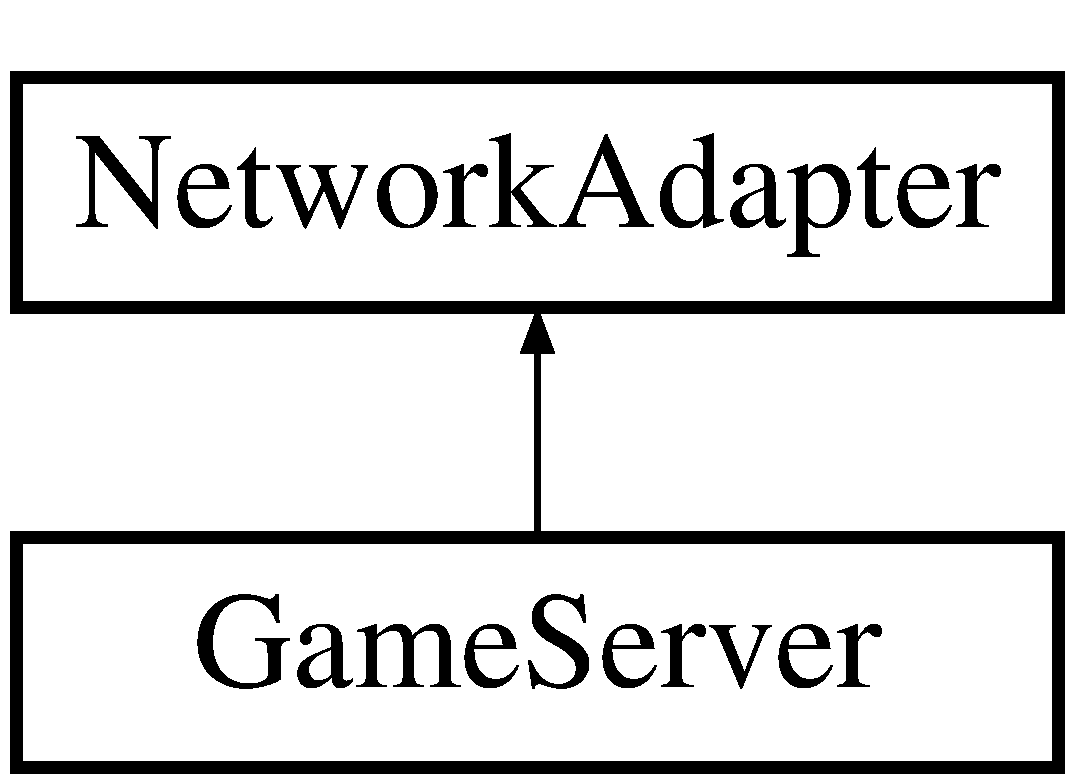
\includegraphics[height=2.000000cm]{classGameServer}
\end{center}
\end{figure}
\subsection*{\-Public \-Slots}
\begin{DoxyCompactItemize}
\item 
\hypertarget{classGameServer_ae41954b45bd6e4f7cff0b9c9034206cc}{void \hyperlink{classGameServer_ae41954b45bd6e4f7cff0b9c9034206cc}{new\-Connection} ()}\label{classGameServer_ae41954b45bd6e4f7cff0b9c9034206cc}

\begin{DoxyCompactList}\small\item\em called when a new client connects \end{DoxyCompactList}\item 
\hypertarget{classGameServer_ae04551b358465ca81a34073abb7d6380}{void \hyperlink{classGameServer_ae04551b358465ca81a34073abb7d6380}{read\-Ready} ()}\label{classGameServer_ae04551b358465ca81a34073abb7d6380}

\begin{DoxyCompactList}\small\item\em called when new data is available from the client \end{DoxyCompactList}\end{DoxyCompactItemize}
\subsection*{\-Public \-Member \-Functions}
\begin{DoxyCompactItemize}
\item 
\hypertarget{classGameServer_a23246629b4e19dcd029ad89455147461}{{\bfseries \-Game\-Server} (\-Q\-Object $\ast$parent=0)}\label{classGameServer_a23246629b4e19dcd029ad89455147461}

\item 
\hypertarget{classGameServer_a65f06eb193e2ce2670f1b2f65c0a7469}{void {\bfseries init} ()}\label{classGameServer_a65f06eb193e2ce2670f1b2f65c0a7469}

\item 
\hypertarget{classGameServer_a58e009e4c2444745fb86a4085a0ab376}{void {\bfseries send} (\-Q\-String data)}\label{classGameServer_a58e009e4c2444745fb86a4085a0ab376}

\end{DoxyCompactItemize}


\subsection{\-Detailed \-Description}
\-Class that handles server client connection. 

\-Class that handles server client connection

\begin{DoxyAuthor}{\-Author}
\-Roland \-Luckenthuber 

\-Denis \-Neuling 
\end{DoxyAuthor}


\-The documentation for this class was generated from the following files\-:\begin{DoxyCompactItemize}
\item 
gameserver.\-h\item 
gameserver.\-cpp\end{DoxyCompactItemize}

\hypertarget{classHelper}{\section{\-Helper \-Class \-Reference}
\label{classHelper}\index{\-Helper@{\-Helper}}
}


\hyperlink{classHelper}{\-Helper} class for \-Connect \-Four.  




{\ttfamily \#include $<$helper.\-h$>$}

\subsection*{\-Static \-Public \-Member \-Functions}
\begin{DoxyCompactItemize}
\item 
\hypertarget{classHelper_a13ac9ee4039795a9b27bc38a81b9f870}{static \-Q\-String {\bfseries board\-Update} ()}\label{classHelper_a13ac9ee4039795a9b27bc38a81b9f870}

\item 
\hypertarget{classHelper_ae7ae04b5ed393589228994c9ce203cac}{static void {\bfseries \-Draw\-Circle} (float radius)}\label{classHelper_ae7ae04b5ed393589228994c9ce203cac}

\item 
\hypertarget{classHelper_a41d44186f3a08524419153f19aa9b5f2}{static \-Q\-Color {\bfseries \-Get\-Coin\-Color} (\-Coin coin)}\label{classHelper_a41d44186f3a08524419153f19aa9b5f2}

\item 
\hypertarget{classHelper_aeb6829bbdecf8901d143d6a364082919}{static \-Q\-String {\bfseries \-Coin\-To\-String} (\-Coin coin)}\label{classHelper_aeb6829bbdecf8901d143d6a364082919}

\item 
\hypertarget{classHelper_a665cf4e080d1e25199e5545df0cc253c}{static \-Q\-String {\bfseries \-Result\-To\-String} (\-Result game)}\label{classHelper_a665cf4e080d1e25199e5545df0cc253c}

\end{DoxyCompactItemize}


\subsection{\-Detailed \-Description}
\hyperlink{classHelper}{\-Helper} class for \-Connect \-Four. 

\hyperlink{classHelper}{\-Helper} class for \-Connect \-Four

\begin{DoxyAuthor}{\-Author}
\-Roland \-Luckenthuber 

\-Denis \-Neuling 
\end{DoxyAuthor}


\-The documentation for this class was generated from the following file\-:\begin{DoxyCompactItemize}
\item 
helper.\-h\end{DoxyCompactItemize}

\hypertarget{classMainWindow}{\section{\-Main\-Window \-Class \-Reference}
\label{classMainWindow}\index{\-Main\-Window@{\-Main\-Window}}
}


main window class  




{\ttfamily \#include $<$mainwindow.\-h$>$}

\subsection*{\-Public \-Member \-Functions}
\begin{DoxyCompactItemize}
\item 
\hypertarget{classMainWindow_a8b244be8b7b7db1b08de2a2acb9409db}{{\bfseries \-Main\-Window} (\-Q\-Widget $\ast$parent=0)}\label{classMainWindow_a8b244be8b7b7db1b08de2a2acb9409db}

\item 
\hypertarget{classMainWindow_af747387b0953cbb422b3cb52031b863c}{\-Q\-Size {\bfseries size} ()}\label{classMainWindow_af747387b0953cbb422b3cb52031b863c}

\item 
\hypertarget{classMainWindow_a781737f6e3b1f3e97e6a7eebb6396771}{\-Q\-Size {\bfseries size\-Hint} () const }\label{classMainWindow_a781737f6e3b1f3e97e6a7eebb6396771}

\end{DoxyCompactItemize}


\subsection{\-Detailed \-Description}
main window class 

application's main window

\begin{DoxyAuthor}{\-Author}
\-Roland \-Luckenthuber 

\-Denis \-Neuling 
\end{DoxyAuthor}


\-The documentation for this class was generated from the following files\-:\begin{DoxyCompactItemize}
\item 
mainwindow.\-h\item 
mainwindow.\-cpp\end{DoxyCompactItemize}

\hypertarget{classMinMax}{\section{\-Min\-Max \-Class \-Reference}
\label{classMinMax}\index{\-Min\-Max@{\-Min\-Max}}
}


\-Negamax algorithm.  




{\ttfamily \#include $<$minmax.\-h$>$}

\subsection*{\-Public \-Member \-Functions}
\begin{DoxyCompactItemize}
\item 
\hypertarget{classMinMax_a0727d40296556cb72e6b147796e9cb06}{int \hyperlink{classMinMax_a0727d40296556cb72e6b147796e9cb06}{calculate\-Move} (\hyperlink{classGameBoard}{\-Game\-Board} \&board, \hyperlink{classGameManager}{\-Game\-Manager} \&manager)}\label{classMinMax_a0727d40296556cb72e6b147796e9cb06}

\begin{DoxyCompactList}\small\item\em calculares the ai's nex move \end{DoxyCompactList}\end{DoxyCompactItemize}


\subsection{\-Detailed \-Description}
\-Negamax algorithm. 

\-Negamax algorithm

\begin{DoxyAuthor}{\-Author}
\-Roland \-Luckenthuber 

\-Denis \-Neuling
\end{DoxyAuthor}
\hyperlink{}{http\-://en.\-wikipedia.\-org/wiki/\-Negamax}

\-The documentation for this class was generated from the following file\-:\begin{DoxyCompactItemize}
\item 
minmax.\-h\end{DoxyCompactItemize}

\hypertarget{classNetworkAdapter}{\section{\-Network\-Adapter \-Class \-Reference}
\label{classNetworkAdapter}\index{\-Network\-Adapter@{\-Network\-Adapter}}
}


base class for a network connection (server and client)  




{\ttfamily \#include $<$networkadapter.\-h$>$}

\-Inheritance diagram for \-Network\-Adapter\-:\begin{figure}[H]
\begin{center}
\leavevmode
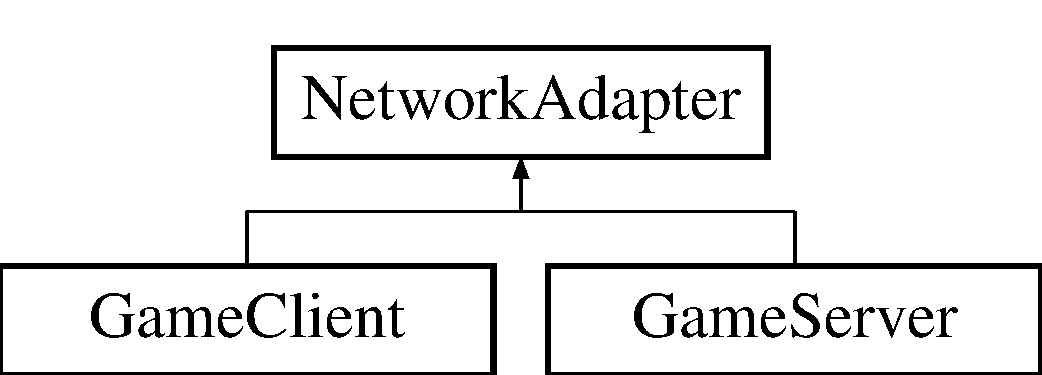
\includegraphics[height=2.000000cm]{classNetworkAdapter}
\end{center}
\end{figure}
\subsection*{\-Signals}
\begin{DoxyCompactItemize}
\item 
\hypertarget{classNetworkAdapter_a2da2230a1cdf125105537d7a5b143bd0}{void \hyperlink{classNetworkAdapter_a2da2230a1cdf125105537d7a5b143bd0}{connection\-Established} ()}\label{classNetworkAdapter_a2da2230a1cdf125105537d7a5b143bd0}

\begin{DoxyCompactList}\small\item\em triggered after a new connection has been established either by server or client \end{DoxyCompactList}\item 
\hypertarget{classNetworkAdapter_ac2e6cce84f774b166dfda66e98ee655e}{void \hyperlink{classNetworkAdapter_ac2e6cce84f774b166dfda66e98ee655e}{data\-Received} (const \-Q\-String \&data)}\label{classNetworkAdapter_ac2e6cce84f774b166dfda66e98ee655e}

\begin{DoxyCompactList}\small\item\em triggered after new data is available on the socket \end{DoxyCompactList}\end{DoxyCompactItemize}
\subsection*{\-Public \-Member \-Functions}
\begin{DoxyCompactItemize}
\item 
\hypertarget{classNetworkAdapter_a06f7164599740e840ef4663558019319}{{\bfseries \-Network\-Adapter} (\-Q\-Object $\ast$parent=0)}\label{classNetworkAdapter_a06f7164599740e840ef4663558019319}

\item 
\hypertarget{classNetworkAdapter_a5bfaa6d0344e0026418c99a27548a332}{virtual void {\bfseries init} ()=0}\label{classNetworkAdapter_a5bfaa6d0344e0026418c99a27548a332}

\item 
\hypertarget{classNetworkAdapter_a304921c7d4e599031608a9a9217c900f}{virtual void {\bfseries send} (\-Q\-String data)=0}\label{classNetworkAdapter_a304921c7d4e599031608a9a9217c900f}

\item 
\hypertarget{classNetworkAdapter_a37549ba9c99061a8c5407299b380139d}{bool {\bfseries \-Is\-Server} ()}\label{classNetworkAdapter_a37549ba9c99061a8c5407299b380139d}

\end{DoxyCompactItemize}
\subsection*{\-Protected \-Attributes}
\begin{DoxyCompactItemize}
\item 
\hypertarget{classNetworkAdapter_a8517d41d27fad01cd65a6342b562f7e0}{bool {\bfseries m\-\_\-\-Is\-Server}}\label{classNetworkAdapter_a8517d41d27fad01cd65a6342b562f7e0}

\item 
\hypertarget{classNetworkAdapter_a805305b01405a2890d9bbb784d44bde1}{\-Q\-Tcp\-Socket $\ast$ {\bfseries m\-\_\-p\-Socket}}\label{classNetworkAdapter_a805305b01405a2890d9bbb784d44bde1}

\end{DoxyCompactItemize}


\subsection{\-Detailed \-Description}
base class for a network connection (server and client) 

\-The documentation for this class was generated from the following files\-:\begin{DoxyCompactItemize}
\item 
networkadapter.\-h\item 
networkadapter.\-cpp\end{DoxyCompactItemize}

\hypertarget{classPlayer}{\section{\-Player \-Class \-Reference}
\label{classPlayer}\index{\-Player@{\-Player}}
}


player data holder  




{\ttfamily \#include $<$player.\-h$>$}

\subsection*{\-Public \-Member \-Functions}
\begin{DoxyCompactItemize}
\item 
\hypertarget{classPlayer_a877063d8943797400d52fe2735d521c3}{{\bfseries \-Player} (\-Q\-String name, \-Coin color, bool is\-Ai\-Player=false)}\label{classPlayer_a877063d8943797400d52fe2735d521c3}

\item 
\hypertarget{classPlayer_a60bab4053f47b075a4228b5237394711}{\-Coin {\bfseries get\-Coin} ()}\label{classPlayer_a60bab4053f47b075a4228b5237394711}

\item 
\hypertarget{classPlayer_ade0334ac0e87ac1c5e09ce78f2cafd83}{\-Q\-String {\bfseries get\-Name} ()}\label{classPlayer_ade0334ac0e87ac1c5e09ce78f2cafd83}

\item 
\hypertarget{classPlayer_a0f345ac8c69275c700ed776ddac094c3}{bool {\bfseries is\-Ai\-Player} ()}\label{classPlayer_a0f345ac8c69275c700ed776ddac094c3}

\end{DoxyCompactItemize}


\subsection{\-Detailed \-Description}
player data holder 

class representing a player

\begin{DoxyAuthor}{\-Author}
\-Roland \-Luckenthuber 

\-Denis \-Neuling 
\end{DoxyAuthor}


\-The documentation for this class was generated from the following file\-:\begin{DoxyCompactItemize}
\item 
player.\-h\end{DoxyCompactItemize}

\hypertarget{classRenderObject}{\section{\-Render\-Object \-Class \-Reference}
\label{classRenderObject}\index{\-Render\-Object@{\-Render\-Object}}
}


abstract class for each renderable object  




{\ttfamily \#include $<$renderobject.\-h$>$}

\-Inheritance diagram for \-Render\-Object\-:\begin{figure}[H]
\begin{center}
\leavevmode
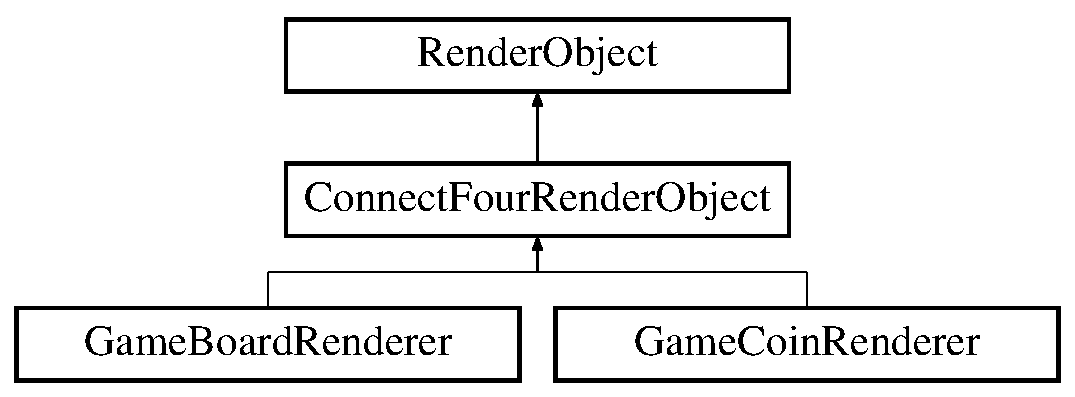
\includegraphics[height=3.000000cm]{classRenderObject}
\end{center}
\end{figure}
\subsection*{\-Public \-Member \-Functions}
\begin{DoxyCompactItemize}
\item 
\hypertarget{classRenderObject_ac4cc404d2bada4f6652b94cdaa833502}{virtual void {\bfseries init} ()}\label{classRenderObject_ac4cc404d2bada4f6652b94cdaa833502}

\item 
\hypertarget{classRenderObject_aa4578bf61a73304b8613727cd89ee576}{virtual void {\bfseries draw} ()=0}\label{classRenderObject_aa4578bf61a73304b8613727cd89ee576}

\item 
\hypertarget{classRenderObject_a46fffcc84648ad62836cab723c8c1f58}{virtual void {\bfseries resize} (int width, int height)=0}\label{classRenderObject_a46fffcc84648ad62836cab723c8c1f58}

\end{DoxyCompactItemize}


\subsection{\-Detailed \-Description}
abstract class for each renderable object 

\-The documentation for this class was generated from the following file\-:\begin{DoxyCompactItemize}
\item 
renderobject.\-h\end{DoxyCompactItemize}

\hypertarget{structSettings}{\section{\-Settings \-Struct \-Reference}
\label{structSettings}\index{\-Settings@{\-Settings}}
}


data holder between ui and game  




{\ttfamily \#include $<$settings.\-h$>$}

\subsection*{\-Public \-Attributes}
\begin{DoxyCompactItemize}
\item 
\hypertarget{structSettings_ac5a707ab0e620e9aeb22d98478197506}{int {\bfseries width}}\label{structSettings_ac5a707ab0e620e9aeb22d98478197506}

\item 
\hypertarget{structSettings_af63a2c25f93b1f54a88f9217e95fbcc0}{int {\bfseries height}}\label{structSettings_af63a2c25f93b1f54a88f9217e95fbcc0}

\item 
\hypertarget{structSettings_a02c5d891df66d91711d7ef348bc0a98a}{\-Q\-String {\bfseries player1}}\label{structSettings_a02c5d891df66d91711d7ef348bc0a98a}

\item 
\hypertarget{structSettings_af36a424cc1c71f670f4e0b221f1ac2d4}{\-Q\-String {\bfseries player2}}\label{structSettings_af36a424cc1c71f670f4e0b221f1ac2d4}

\item 
\hypertarget{structSettings_a5dd01adc93a126d0c4443b9e04906388}{\-Q\-String {\bfseries ip\-Address}}\label{structSettings_a5dd01adc93a126d0c4443b9e04906388}

\item 
\hypertarget{structSettings_a0d2542ef361af07d3a52243c46305541}{bool {\bfseries use\-A\-I}}\label{structSettings_a0d2542ef361af07d3a52243c46305541}

\item 
\hypertarget{structSettings_aa510d772b330cc005608bb764d8aaf2b}{bool {\bfseries ai\-Begins}}\label{structSettings_aa510d772b330cc005608bb764d8aaf2b}

\end{DoxyCompactItemize}


\subsection{\-Detailed \-Description}
data holder between ui and game 

data holder between ui and game

\begin{DoxyAuthor}{\-Author}
\-Roland \-Luckenthuber 

\-Denis \-Neuling 
\end{DoxyAuthor}


\-The documentation for this struct was generated from the following file\-:\begin{DoxyCompactItemize}
\item 
settings.\-h\end{DoxyCompactItemize}

\hypertarget{classSettingsWidget}{\section{\-Settings\-Widget \-Class \-Reference}
\label{classSettingsWidget}\index{\-Settings\-Widget@{\-Settings\-Widget}}
}


widget for settings  




{\ttfamily \#include $<$settingswidget.\-h$>$}

\subsection*{\-Signals}
\begin{DoxyCompactItemize}
\item 
\hypertarget{classSettingsWidget_a0dc3dbbc8b45cae0480cf727ad53c77a}{void {\bfseries start\-Button\-Pressed} (\hyperlink{structSettings}{\-Settings} settings)}\label{classSettingsWidget_a0dc3dbbc8b45cae0480cf727ad53c77a}

\item 
\hypertarget{classSettingsWidget_a3318e4fa37e5fc7aa7b6b272345b9853}{void {\bfseries host\-Server\-Button\-Pressed} (\hyperlink{structSettings}{\-Settings} settings)}\label{classSettingsWidget_a3318e4fa37e5fc7aa7b6b272345b9853}

\item 
\hypertarget{classSettingsWidget_a5d848f32b81af10a30d678816d15fdf4}{void {\bfseries connect\-Button\-Pressed} (\hyperlink{structSettings}{\-Settings} settings)}\label{classSettingsWidget_a5d848f32b81af10a30d678816d15fdf4}

\item 
\hypertarget{classSettingsWidget_a7ee9f48c228d92314768f2e63dcc2b55}{void {\bfseries highscore\-Button\-Pressed} ()}\label{classSettingsWidget_a7ee9f48c228d92314768f2e63dcc2b55}

\end{DoxyCompactItemize}
\subsection*{\-Public \-Member \-Functions}
\begin{DoxyCompactItemize}
\item 
\hypertarget{classSettingsWidget_ab381a630fcf24d7fe49ab7bd2896c052}{{\bfseries \-Settings\-Widget} (\-Q\-Widget $\ast$parent=0)}\label{classSettingsWidget_ab381a630fcf24d7fe49ab7bd2896c052}

\end{DoxyCompactItemize}


\subsection{\-Detailed \-Description}
widget for settings 

widget for settings

\begin{DoxyAuthor}{\-Author}
\-Roland \-Luckenthuber 

\-Denis \-Neuling 
\end{DoxyAuthor}


\-The documentation for this class was generated from the following files\-:\begin{DoxyCompactItemize}
\item 
settingswidget.\-h\item 
settingswidget.\-cpp\end{DoxyCompactItemize}

\hypertarget{classTCPGameManager}{\section{\-T\-C\-P\-Game\-Manager \-Class \-Reference}
\label{classTCPGameManager}\index{\-T\-C\-P\-Game\-Manager@{\-T\-C\-P\-Game\-Manager}}
}


\-Gamemanager that handles \-Network game related tasks.  




{\ttfamily \#include $<$tcpgamemanager.\-h$>$}

\-Inheritance diagram for \-T\-C\-P\-Game\-Manager\-:\begin{figure}[H]
\begin{center}
\leavevmode
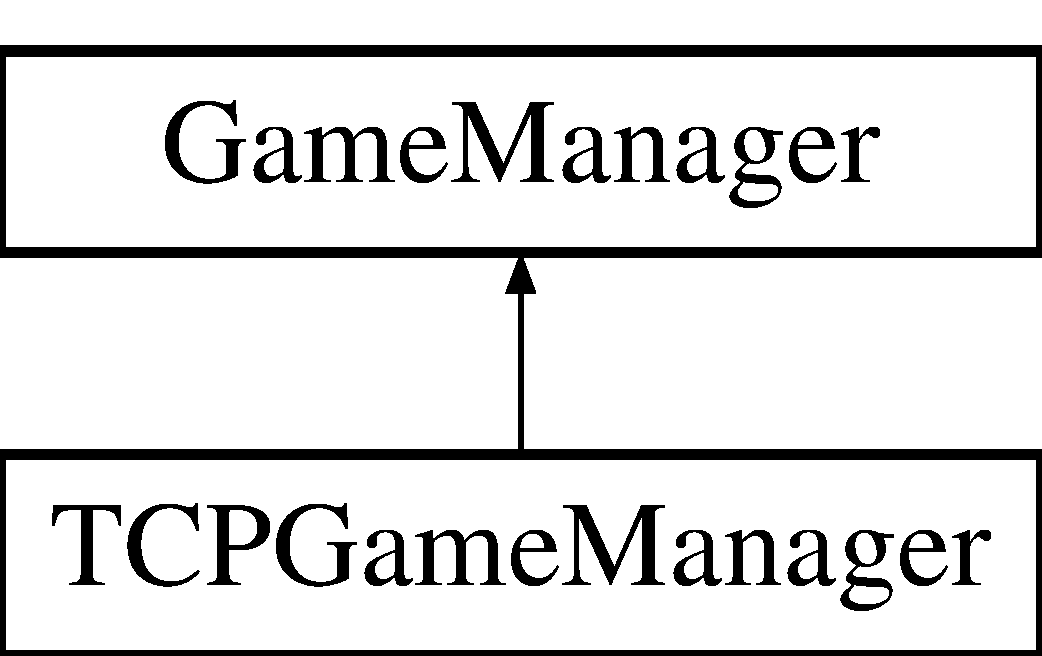
\includegraphics[height=2.000000cm]{classTCPGameManager}
\end{center}
\end{figure}
\subsection*{\-Public \-Slots}
\begin{DoxyCompactItemize}
\item 
\hypertarget{classTCPGameManager_a616b05b986023096f7475e32c70a059d}{void {\bfseries client\-Connected} ()}\label{classTCPGameManager_a616b05b986023096f7475e32c70a059d}

\item 
\hypertarget{classTCPGameManager_a65421be056b0c53a6deed1bd405ffc6b}{void {\bfseries connection\-Established} ()}\label{classTCPGameManager_a65421be056b0c53a6deed1bd405ffc6b}

\item 
\hypertarget{classTCPGameManager_a6412d2d4a43e5ff353d410e810f60675}{void {\bfseries received\-Data} (const \-Q\-String \&data)}\label{classTCPGameManager_a6412d2d4a43e5ff353d410e810f60675}

\end{DoxyCompactItemize}
\subsection*{\-Public \-Member \-Functions}
\begin{DoxyCompactItemize}
\item 
\hypertarget{classTCPGameManager_a0a83c4efd02332883aaa7935b480ec2c}{{\bfseries \-T\-C\-P\-Game\-Manager} (\-Q\-Widget $\ast$parent)}\label{classTCPGameManager_a0a83c4efd02332883aaa7935b480ec2c}

\item 
\hypertarget{classTCPGameManager_a7d4415253458e80a05314f91a0879fd0}{void \hyperlink{classTCPGameManager_a7d4415253458e80a05314f91a0879fd0}{start\-Game} (\hyperlink{structSettings}{\-Settings} settings)}\label{classTCPGameManager_a7d4415253458e80a05314f91a0879fd0}

\begin{DoxyCompactList}\small\item\em instanciates renderer and gameboard \end{DoxyCompactList}\end{DoxyCompactItemize}
\subsection*{\-Protected \-Member \-Functions}
\begin{DoxyCompactItemize}
\item 
\hypertarget{classTCPGameManager_af76ec973ba1c3e7f58ac979fffccb85f}{void \hyperlink{classTCPGameManager_af76ec973ba1c3e7f58ac979fffccb85f}{mouse\-Press\-Event} (\-Q\-Mouse\-Event $\ast$event)}\label{classTCPGameManager_af76ec973ba1c3e7f58ac979fffccb85f}

\begin{DoxyCompactList}\small\item\em drop coins and check finish game \end{DoxyCompactList}\end{DoxyCompactItemize}
\subsection*{\-Protected \-Attributes}
\begin{DoxyCompactItemize}
\item 
\hypertarget{classTCPGameManager_aabea99b1b4ed457eff4a5f0db194644b}{bool {\bfseries m\-\_\-\-Network\-Initialized}}\label{classTCPGameManager_aabea99b1b4ed457eff4a5f0db194644b}

\item 
\hypertarget{classTCPGameManager_a762b0b3ae60c0076165843b78d011927}{bool {\bfseries m\-\_\-\-Server\-Turn}}\label{classTCPGameManager_a762b0b3ae60c0076165843b78d011927}

\item 
\hypertarget{classTCPGameManager_ad973154be37079b7510d4ca3d66d47fb}{bool {\bfseries m\-\_\-\-Sent\-But\-Not\-Received}}\label{classTCPGameManager_ad973154be37079b7510d4ca3d66d47fb}

\end{DoxyCompactItemize}


\subsection{\-Detailed \-Description}
\-Gamemanager that handles \-Network game related tasks. 

\-Gamemanager that handles \-Network game related tasks

\begin{DoxyAuthor}{\-Author}
\-Roland \-Luckenthuber 

\-Denis \-Neuling 
\end{DoxyAuthor}


\-The documentation for this class was generated from the following files\-:\begin{DoxyCompactItemize}
\item 
tcpgamemanager.\-h\item 
tcpgamemanager.\-cpp\end{DoxyCompactItemize}

\printindex
\end{document}
